\subsubsection{Road}
\begin{figure}[h]
\centering
\nogloxy{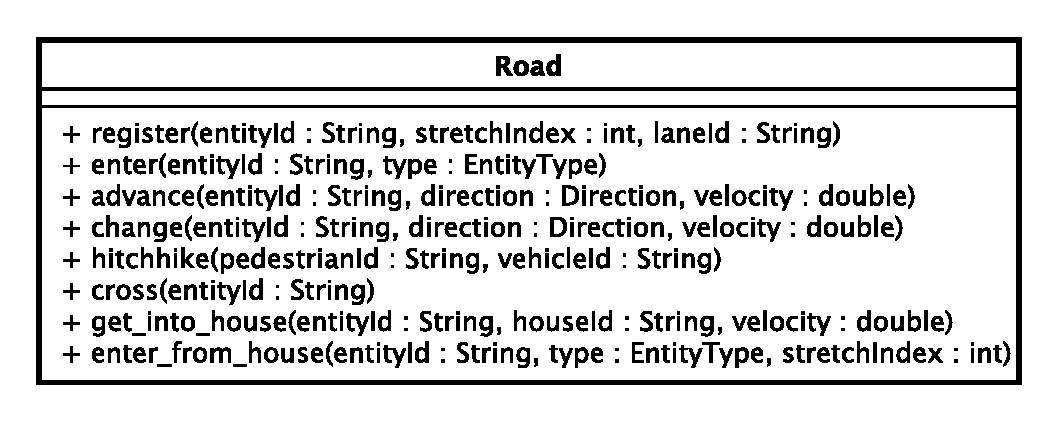
\includegraphics[scale=0.6,keepaspectratio]{diagrams/workspace/application/road.eps}}
\caption{Application::Road}
\end{figure}
\FloatBarrier
A Road is made of stretches and it offers the following operations:
\begin{itemize}
	\item \texttt{register(entityId : String, stretchIndex : int, laneId : String)}
	\\Puts an entity into the stretch having the given index
	\begin{itemize}
		\item \textit{Use}: boostrap phase
	\end{itemize}
	\item \texttt{enter(entityId : String, type : EntityType)}
	\\Puts an entity into the Road in the rightmost lane available for the entity type
	\begin{itemize}
		\item E.g. a car does not land in a sidewalk
	\end{itemize}
	\item \texttt{advance(entityId : String, direction : Direction, velocity : double)}
	\\Moves an entity forward along the Road	
	\begin{itemize}
		\item If a Road end has reached, the entity is notified providing it the adjacent Roads list
		\item The entity velocity is calculated by each stretch taking a specific range of possible values according to the entity type
	\end{itemize}
	\item \texttt{change(entityId : String, direction : Direction, velocity : double)}
	\\Moves an entity to next stretch in the given direction (left or right)	
	\begin{itemize}
		\item If a Road end is reached, it does not allow the lane change and it sends a message for notifying the entity
		\item If no more lanes for the entity type exist in the given direction, it sends a message for notifying the entity
	\end{itemize}
	\item \texttt{hitchhike(pedestrianId : String, vehicleId : String)}
	\\Brings a pedestrian into an vehicle
	\item \texttt{cross(entityId : String)}
	\\Moves a pedestrian or a cyclist to the other side of the Road
	\begin{itemize}
		\item If there is an entity in the stretch near a sidewalk, it books a Road crossing
		\item No vehicles can enter stretches covered by booked zebra crossing
		\item If a stretch near a sidewalk is free (whether it is booked or not), pedestrian can start crossing the Road
	\end{itemize}
	\item \texttt{get\_into\_house(entityId : String, houseId : String, velocity : double)}
	\\Brings an entity into a house accessible from the Road where the entity is
	\begin{itemize}
		\item It brings the entity into the house, if the entity is in a stretch where the given house is accessible. Otherwise, It moves the entity forward at the specified velocity
	\end{itemize}
	\item \texttt{enter\_from\_house(entityId : String, type : EntityType, stretchIndex : int)}
	\\Brings an entity out from a house and it puts the entity into the Road stretch having the given index
	\begin{itemize}
		\item An entity coming out from a house has lower priority than one is already on the Road. So that, before exiting the house, the first one has to wait the other one is passed
	\end{itemize}
\end{itemize}
\paragraph{Remarks}
\ \\A lane change can happen in two cases:
\begin{itemize}
	\item Overtaking. It is requested in a particular stretch
	\item Road change. It is requested in the first stretch of the Road taken
\end{itemize}
We assume a Road is at least $n$ stretches long if it consists of $n$ lanes for motor vehicles.